\documentclass[runningheads]{llncs}

\usepackage[T1]{fontenc}
\usepackage[utf8]{inputenc}
\usepackage{lmodern}
\usepackage{booktabs}
\usepackage{tabularx}
\usepackage{graphicx}
\usepackage{pgfplots}
\pgfplotsset{compat=1.18}
\usepackage{amsmath}
\usepackage{amssymb}
\usepackage{hyperref}
\usepackage{float}
\usepackage{xcolor}
\usepackage{colortbl}
\usepackage{multirow}

\setlength{\tabcolsep}{3pt}

\begin{document}

\title{Supplementary Material:\\ An Explainable Hybrid of Lexicon Rules and Multilingual Transformers for Bilingual Hate Speech Detection}
\titlerunning{Supplementary Material: Hybrid Bilingual Hate Speech Detection}
\author{
Pham Kha Vy\inst{1}
 \and
Cao Hong Nga\inst{1}\textsuperscript{(*)}
\and
Jia-Ching Wang\inst{2}\textsuperscript{(*)}
}

\authorrunning{K. V. Pham, H. N. Cao, and J. C. Wang}
\institute{
FPT University, Can Tho, Vietnam\\
\email{phamkhavycm2004@gmail.com}, \email{caohongnga@gmail.com}
\and
Department of Computer Science \& Information Engineering, National Central University, Taoyuan, Taiwan\\
\email{jcw@csie.ncu.edu.tw}\\
\textsuperscript{(*)}is the correspondent author.
}
\maketitle

\section{Overview of Supplementary Experiments}
This document provides supplementary materials for the ICCIES 2027 paper (15-page main manuscript). It details exhaustive per-component experimental evaluations, including language routing, lexicon rule ablation, neural backbone comparisons, decision-level fusion, end-to-end pipeline benchmarks, latency breakdowns, surface form robustness, error overlap, and paired statistical significance testing (bootstrap and McNemar tests). All reported empirical figures are extracted directly from frozen evaluation outputs stored in \texttt{outputs/evaluation/}.

\section{Language Detection and Routing}
\subsection{Language Routing Confusion Matrix}
Table~\ref{tab:langid_full} presents the confusion matrix for the language router evaluated across the 9,158-sample bilingual test stream (6,680 ViHSD comments + 2,478 Davidson comments).

\begin{table}[H]
\centering
\caption{Language detection routing confusion matrix ($n=9{,}158$). Rows: Actual ground-truth language; Columns: Router output decision.}
\label{tab:langid_full}
\scriptsize
\setlength{\tabcolsep}{2pt}
\resizebox{\textwidth}{!}{%
\begin{tabular}{lrrrrr}
\toprule
Actual Language & Predicted VI & Predicted EN & Predicted Mix & Predicted Multi. & Total \\
\midrule
Vietnamese & 6,278 & 58 & 27 & 317 & 6,680 \\
English & 4 & 2,341 & 4 & 129 & 2,478 \\
\midrule
\textbf{Total} & \textbf{6,282} & \textbf{2,399} & \textbf{31} & \textbf{446} & \textbf{9,158} \\
\bottomrule
\end{tabular}%
}
\end{table}

\subsection{Language Detection Accuracy on Clean Held-out Sets}
Table~\ref{tab:langid_robustness} reports routing accuracy on the clean ViNLI (Vietnamese) and Wortschatz (English) held-out sets used for the language detection benchmark.

\begin{table}[H]
\centering
\caption{Language detection accuracy on clean held-out sets (ViNLI Vietnamese, $n=29{,}934$; Wortschatz English Leipzig 2015, $n=29{,}934$).}
\label{tab:langid_robustness}
\begin{tabular}{lrr}
\toprule
Test Set & $N$ & Detection Accuracy (\%) \\
\midrule
ViNLI (Vietnamese) & 29,934 & 99.97\% \\
Wortschatz (English) & 29,934 & 99.64\% \\
\midrule
\textbf{Overall} & \textbf{59,868} & \textbf{99.81\%} \\
\bottomrule
\end{tabular}
\end{table}

\subsection{Routing Latency Breakdown}
Table~\ref{tab:langid_latency} details the latency profile for the language routing stage. The Language Router row is measured on the combined ViNLI + Wortschatz clean benchmark ($n=59{,}868$); the AI Backbone and Total rows retain the original 9,158-stream measurements.

\begin{table}[H]
\centering
\caption{Routing latency breakdown (Language Router row on ViNLI+Wortschatz clean benchmark, $n=59{,}868$).}
\label{tab:langid_latency}
\scriptsize
\setlength{\tabcolsep}{2pt}
\resizebox{\textwidth}{!}{%
\begin{tabular}{lccccc}
\toprule
Stage & Mean (ms) & P50 (ms) & P95 (ms) & P99 (ms) & Throughput (texts/s) \\
\midrule
Language Router (langID) & 1.668 & 1.633 & 1.898 & 2.165 & 599.5 \\
AI Backbone Pipeline & 3.990 & --- & --- & --- & 250.6 \\
\midrule
\textbf{Total Serialised Pipeline} & \textbf{5.658} & --- & --- & --- & --- \\
\bottomrule
\end{tabular}%
}
\end{table}

\begin{figure}[H]
\centering
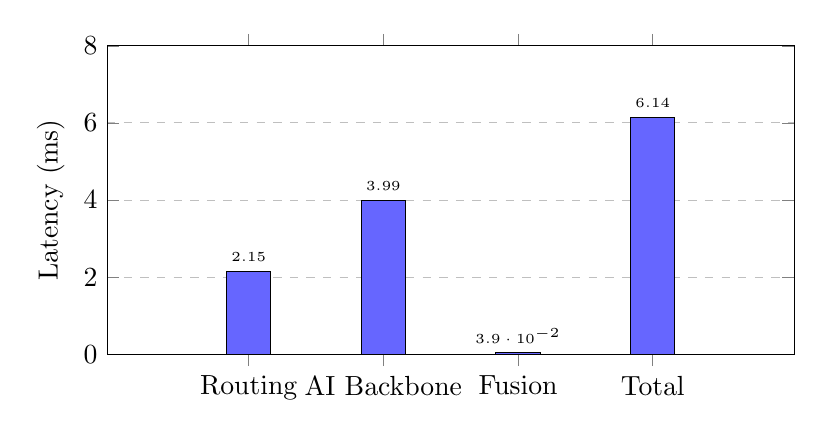
\begin{tikzpicture}
\begin{axis}[
    ybar,
    enlarge x limits=0.35,
    ylabel={Latency (ms)},
    symbolic x coords={Routing,AI Backbone,Fusion,Total},
    xtick=data,
    nodes near coords,
    nodes near coords align={vertical},
    every node near coord/.append style={font=\tiny\bfseries},
    ymin=0, ymax=8,
    width=0.85\textwidth,
    height=5.5cm,
    bar width=16pt,
    ymajorgrids=true,
    grid style=dashed,
]
\addplot[fill=blue!60] coordinates {(Routing,2.153) (AI Backbone,3.990) (Fusion,0.039) (Total,6.143)};
\end{axis}
\end{tikzpicture}
\caption{Latency breakdown by pipeline stage on the bilingual test stream ($n=9{,}158$).}
\label{fig:latency_breakdown}
\end{figure}

\section{Rule Engine Component Ablation Study}
\subsection{Component Contribution Evaluation}
Table~\ref{tab:rule_ablation_full} reports component ablation metrics for the Vietnamese Lexicon Rule Engine evaluated on the ViHSD test split ($n=6{,}680$). Each variant disables one rule mechanism, re-tunes thresholds on validation, and scores test once.

\begin{table}[H]
\centering
\caption{Vietnamese Lexicon Rule Engine component ablation study on ViHSD test ($n=6{,}680$).}
\label{tab:rule_ablation_full}
\begin{tabular}{lcccc}
\toprule
Variant & Accuracy & Macro-F1 & HATE F1 & $\Delta$Macro-F1 vs Full \\
\midrule
Full Rule Engine & 0.8774 & 0.6602 & 0.5906 & --- \\
No Entry Confidence & 0.8781 & 0.6610 & 0.5935 & +0.0008 \\
No Context Matching & 0.8774 & 0.6602 & 0.5906 & 0.0000 \\
No Obfuscation Views & 0.8772 & 0.6590 & 0.5896 & -0.0012 \\
No Severity Scaling & 0.8774 & 0.6602 & 0.5906 & 0.0000 \\
\bottomrule
\end{tabular}
\end{table}

\subsection{Detailed Rule Engine Confusion Matrices}
Table~\ref{tab:rule_confusion} illustrates misclassification patterns across rule engine variants on ViHSD test.

\begin{table}[H]
\centering
\caption{Detailed confusion matrix breakdown for standalone Rule Engine variants on ViHSD test ($n=6{,}680$).}
\label{tab:rule_confusion}
\scriptsize
\setlength{\tabcolsep}{2pt}
\resizebox{\textwidth}{!}{%
\begin{tabular}{lrrrr}
\toprule
Rule Variant & HATE $\to$ HATE & HATE $\to$ OFF & HATE $\to$ CLEAN & OFF $\to$ CLEAN \\
\midrule
Full (argmax) & 348 & 0 & 340 & 272 \\
No Fuzzy Matching & 348 & 0 & 340 & 272 \\
No Diacritics Match & 210 & 160 & 318 & 259 \\
No Normalisation & 0 & 0 & 688 & 444 \\
\midrule
Full + Frozen Thresholds & 210 & 160 & 318 & 259 \\
\bottomrule
\end{tabular}%
}
\end{table}

\subsection{Per-Class Metrics for Rule Engine}
Table~\ref{tab:rule_per_class} presents class-wise precision, recall, and F1 scores for rule engine configurations.

\begin{table}[H]
\centering
\caption{Per-class precision, recall, and F1 metrics for standalone Rule Engine configurations on ViHSD test.}
\label{tab:rule_per_class}
\small
\setlength{\tabcolsep}{2pt}
\resizebox{\textwidth}{!}{%
\begin{tabular}{lccccc}
\toprule
Configuration & HATE Precision & HATE Recall & HATE F1 & OFF F1 & CLEAN F1 \\
\midrule
Full Engine (argmax) & 0.469 & 0.506 & 0.487 & 0.000 & 0.927 \\
Full Engine (thresholds) & 0.625 & 0.305 & 0.410 & 0.239 & 0.928 \\
\bottomrule
\end{tabular}%
}
\end{table}

\section{Neural Backbone Model Analysis}
\subsection{Vietnamese Backbone Models}
Table~\ref{tab:vi_backbones_full} summarizes standalone test performance across six Vietnamese Transformer backbones on ViHSD test ($n=6{,}680$).

\begin{table}[H]
\centering
\caption{Performance comparison of Vietnamese mDeBERTa-v3 backbones on ViHSD test ($n=6{,}680$).}
\label{tab:vi_backbones_full}
\scriptsize
\setlength{\tabcolsep}{2pt}
\resizebox{\textwidth}{!}{%
\begin{tabular}{lccccc}
\toprule
Model Identifier & Accuracy & Macro-F1 & HATE F1 & OFF F1 & ECE \\
\midrule
M1 (\texttt{sensitiveai-vi}) & 0.8734 & 0.6545 & 0.5864 & 0.4367 & 0.106 \\
M2 (\texttt{sensitiveai-vi-custom}) & 0.8762 & 0.6575 & 0.5830 & 0.4493 & 0.111 \\
M3 (\texttt{sensitiveai-vi-customdlr2stage}) & 0.8754 & 0.6638 & 0.5943 & 0.4561 & 0.120 \\
M4 (\texttt{sensitiveai-vi-custom-curriculum}) & 0.8731 & 0.6590 & 0.5847 & 0.4535 & 0.119 \\
M5 (\texttt{sensitiveai-vi-customdlr2stage-ext}) & 0.8783 & 0.6536 & 0.5843 & 0.4350 & 0.118 \\
M6 (\texttt{sensitiveai-vi-stage2}) & 0.8633 & 0.6604 & 0.6088 & 0.4382 & 0.068 \\
\bottomrule
\end{tabular}%
}
\end{table}

\subsection{English Backbone Models}
Table~\ref{tab:en_backbones_full} evaluates English Transformer backbones fine-tuned on the Davidson test split ($n=2{,}478$).

\begin{table}[H]
\centering
\caption{Performance comparison of English backbones on Davidson test ($n=2{,}478$).}
\label{tab:en_backbones_full}
\scriptsize
\setlength{\tabcolsep}{2pt}
\resizebox{\textwidth}{!}{%
\begin{tabular}{lccccc}
\toprule
Model Identifier & Accuracy & Macro-F1 & HATE F1 & OFF F1 & CLEAN F1 \\
\midrule
\texttt{sensitiveai-en} & 0.9031 & 0.7676 & 0.4554 & 0.9410 & 0.9063 \\
\texttt{sensitiveai-en-custom} & 0.9031 & 0.7587 & 0.4377 & 0.9404 & 0.8980 \\
\texttt{sensitiveai-en-custom-curriculum} & 0.9072 & 0.7441 & 0.3908 & 0.9445 & 0.8970 \\
\texttt{sensitiveai-en-customdlr2stage} & 0.9108 & 0.7509 & 0.4048 & 0.9457 & 0.9024 \\
\texttt{sensitiveai-en-stage2} & 0.9080 & 0.7722 & 0.4656 & 0.9440 & 0.9070 \\
\bottomrule
\end{tabular}%
}
\end{table}

\subsection{ROC-AUC and Average Precision Performance}
Table~\ref{tab:roc_ap_full} details multi-class ROC-AUC metrics across representative backbone checkpoints.

\begin{table}[H]
\centering
\caption{Class-wise ROC-AUC scores evaluated on ViHSD test split ($n=6{,}680$).}
\label{tab:roc_ap_full}
\scriptsize
\setlength{\tabcolsep}{2pt}
\resizebox{\textwidth}{!}{%
\begin{tabular}{lcccc}
\toprule
Model Checkpoint & HATE ROC-AUC & OFF ROC-AUC & CLEAN ROC-AUC & Macro ROC-AUC \\
\midrule
\texttt{sensitiveai-vi-custom-curriculum} & 0.8949 & 0.8638 & 0.8924 & 0.8837 \\
\texttt{sensitiveai-vi-customdlr2stage} & 0.8966 & 0.8635 & 0.8924 & 0.8842 \\
\texttt{sensitiveai-vi-custom} & 0.8951 & 0.8640 & 0.8920 & 0.8837 \\
\bottomrule
\end{tabular}%
}
\end{table}

\section{Decision-Level Fusion Variants}
\subsection{Comprehensive Decision Strategy Comparison}
Table~\ref{tab:fusion_full} compares all evaluated decision-level fusion strategies on ViHSD test using the frozen \texttt{sensitiveai-vi-custom} backbone.

\begin{table}[H]
\centering
\caption{Comprehensive evaluation of decision fusion rules on ViHSD test ($n=6{,}680$).}
\label{tab:fusion_full}
\scriptsize
\setlength{\tabcolsep}{2pt}
\resizebox{\textwidth}{!}{%
\begin{tabular}{lccccc}
\toprule
Decision Strategy & Accuracy & Macro-F1 & HATE F1 & OFF F1 & CLEAN F1 \\
\midrule
AI-only (argmax) & 0.8762 & 0.6575 & 0.5830 & 0.4493 & 0.9403 \\
Rule-only (argmax) & 0.8494 & 0.4714 & 0.4867 & 0.0000 & 0.9274 \\
Rule-only (frozen thresholds) & 0.8421 & 0.5258 & 0.4102 & 0.2389 & 0.9284 \\
\midrule
Fusion, global $\alpha$ (argmax) & 0.8769 & 0.6583 & 0.5851 & 0.4490 & 0.9408 \\
Fusion, global $\alpha$ (thresholds) & 0.8769 & 0.6583 & 0.5851 & 0.4490 & 0.9408 \\
Fusion, logistic meta-classifier & 0.8624 & 0.6511 & 0.5815 & 0.4379 & 0.9340 \\
Fusion, per-channel $\alpha$ (argmax) & 0.8774 & 0.6593 & 0.5882 & 0.4488 & 0.9408 \\
Fusion, per-channel $\alpha$ + thresholds & 0.8774 & \textbf{0.6602} & 0.5906 & 0.4494 & 0.9407 \\
\bottomrule
\end{tabular}%
}
\end{table}

\subsection{Calibration Diagnostics (ECE, Brier, NLL)}
Table~\ref{tab:calibration_full} summarizes probability calibration metrics across system configurations.

\begin{table}[H]
\centering
\caption{Calibration diagnostics (ECE, Brier score, Negative Log-Likelihood, mean confidence) across evaluation splits.}
\label{tab:calibration_full}
\begin{tabular}{lccccc}
\toprule
System Variant & ECE $\downarrow$ & Brier $\downarrow$ & NLL $\downarrow$ & Mean Conf. & Macro-F1 $\uparrow$ \\
\midrule
AI-only (ViHSD test) & 0.112 & 0.240 & 0.825 & 0.984 & 0.660 \\
Hybrid Fusion (ViHSD test) & 0.092 & 0.230 & 0.822 & 0.939 & 0.660 \\
Uniform Control ($\alpha=0.70$) & 0.092 & 0.227 & --- & 0.791 & 0.658 \\
Mixed E2E Stream ($n=9{,}158$) & 0.078 & 0.230 & 0.755 & 0.904 & 0.779 \\
\midrule
AI-only M3 ($n=6{,}680$) & 0.106 & 0.228 & 0.622 & 0.979 & 0.655 \\
Hybrid M3 ($n=6{,}680$) & 0.068 & 0.217 & 0.482 & 0.931 & 0.660 \\
\bottomrule
\end{tabular}
\end{table}

\begin{figure}[H]
\centering
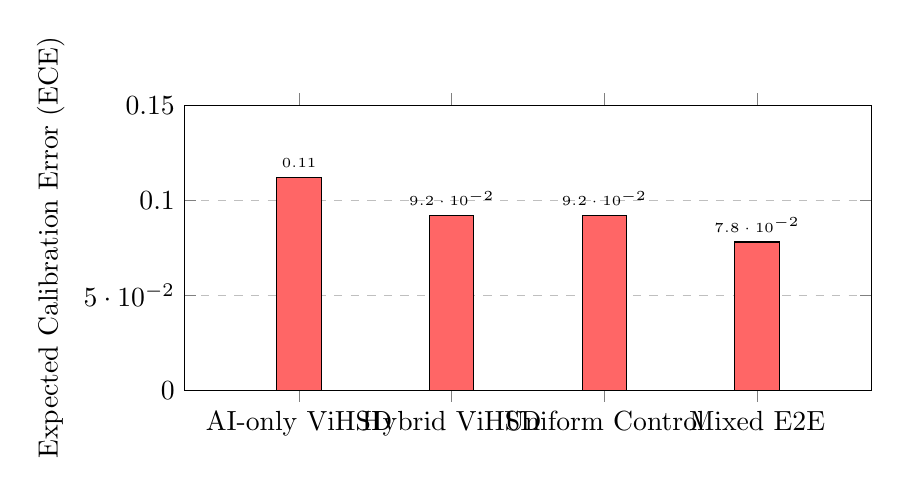
\begin{tikzpicture}
\begin{axis}[
    ybar,
    enlarge x limits=0.25,
    ylabel={Expected Calibration Error (ECE)},
    symbolic x coords={AI-only ViHSD,Hybrid ViHSD,Uniform Control,Mixed E2E},
    xtick=data,
    nodes near coords,
    nodes near coords align={vertical},
    every node near coord/.append style={font=\tiny\bfseries},
    ymin=0, ymax=0.15,
    width=0.85\textwidth,
    height=5.2cm,
    bar width=16pt,
    ymajorgrids=true,
    grid style=dashed,
]
\addplot[fill=red!60] coordinates {(AI-only ViHSD,0.112) (Hybrid ViHSD,0.092) (Uniform Control,0.092) (Mixed E2E,0.078)};
\end{axis}
\end{tikzpicture}
\caption{Expected Calibration Error (ECE) comparison between AI-only, Hybrid, and baseline control variants.}
\label{fig:ece_comparison}
\end{figure}

\section{End-to-End Pipeline Performance}
\subsection{Full End-to-End Benchmark Results}
Table~\ref{tab:e2e_detailed_full} provides complete end-to-end performance metrics over the 9,158 bilingual test stream.

\begin{table}[H]
\centering
\caption{Full end-to-end pipeline benchmark on the bilingual test split ($n=9{,}158$).}
\label{tab:e2e_detailed_full}
\begin{tabular}{llcccc}
\toprule
Execution Mode & Stream / Language & $N$ & Accuracy & Macro-F1 & ECE \\
\midrule
Backbone-only & Vietnamese (ViHSD) & 6,680 & 0.8713 & 0.6602 & 0.112 \\
Backbone-only & English (Davidson) & 2,478 & 0.8717 & 0.7273 & 0.110 \\
\midrule
AI argmax E2E & Bilingual Stream & 9,158 & 0.8714 & 0.7792 & 0.101 \\
AI thresholds E2E & Bilingual Stream & 9,158 & 0.8719 & 0.7803 & 0.101 \\
Hybrid E2E Pipeline & Bilingual Stream & \textbf{9,158} & \textbf{0.8728} & \textbf{0.7787} & \textbf{0.078} \\
\midrule
AI argmax Oracle & Bilingual Stream & 9,158 & 0.8812 & 0.7898 & 0.092 \\
AI thresholds Oracle & Bilingual Stream & 9,158 & 0.8817 & 0.7910 & 0.093 \\
Hybrid Oracle & Bilingual Stream & 9,158 & 0.8826 & 0.7896 & 0.070 \\
\bottomrule
\end{tabular}
\end{table}

\subsection{Per-Language Breakdown of Hybrid E2E}
Table~\ref{tab:e2e_per_lang} breaks down Hybrid E2E results per constituent language split.

\begin{table}[H]
\centering
\caption{Language-stratified metrics for Hybrid E2E pipeline vs Oracle routing baselines.}
\label{tab:e2e_per_lang}
\scriptsize
\setlength{\tabcolsep}{2pt}
\resizebox{\textwidth}{!}{%
\begin{tabular}{lrrrrrr}
\toprule
Evaluation Split & $N$ & Accuracy & Macro-F1 & HATE F1 & OFF F1 & CLEAN F1 \\
\midrule
Vietnamese (Hybrid E2E) & 6,680 & 0.8732 & 0.6603 & 0.6098 & 0.4322 & 0.9388 \\
English (Hybrid E2E) & 2,478 & 0.8717 & 0.7313 & 0.4525 & 0.9196 & 0.8218 \\
\midrule
Vietnamese (AI Oracle) & 6,680 & 0.8711 & 0.6608 & 0.6197 & 0.4251 & 0.9375 \\
English (AI Oracle) & 2,478 & 0.9084 & 0.7676 & 0.4505 & 0.9439 & 0.9083 \\
Vietnamese (Hybrid Oracle) & 6,680 & 0.8731 & 0.6609 & 0.6119 & 0.4320 & 0.9387 \\
English (Hybrid Oracle) & 2,478 & 0.9084 & 0.7726 & 0.4656 & 0.9443 & 0.9081 \\
\bottomrule
\end{tabular}%
}
\end{table}

\subsection{Full Stream Per-Label Performance}
Table~\ref{tab:e2e_per_label_full} presents per-class precision, recall, and F1 across decision modes for the entire stream.

\begin{table}[H]
\centering
\caption{Class-wise performance metrics on the full 9,158-sample bilingual stream.}
\label{tab:e2e_per_label_full}
\small
\begin{tabular}{lrrrrr}
\toprule
Pipeline Mode & Target Class & Precision & Recall & F1-Score & Support ($N$) \\
\midrule
AI argmax E2E & HATE & 0.5931 & 0.5788 & 0.5859 & 831 \\
 & OFFENSIVE & 0.8502 & 0.7981 & 0.8233 & 2,362 \\
 & CLEAN & 0.9158 & 0.9412 & 0.9283 & 5,965 \\
\midrule
AI thresholds E2E & HATE & 0.5889 & 0.5860 & 0.5875 & 831 \\
 & OFFENSIVE & 0.8561 & 0.7959 & 0.8249 & 2,362 \\
 & CLEAN & 0.9157 & 0.9418 & 0.9286 & 5,965 \\
\midrule
Hybrid E2E Pipeline & HATE & 0.5920 & 0.5692 & 0.5804 & 831 \\
 & OFFENSIVE & 0.8592 & 0.7959 & 0.8264 & 2,362 \\
 & CLEAN & 0.9140 & 0.9455 & 0.9295 & 5,965 \\
\bottomrule
\end{tabular}
\end{table}

\subsection{Full Stream Normalized Confusion Matrix}
Table~\ref{tab:e2e_confusion_full} details row-normalized recall confusion for the Hybrid E2E pipeline.

\begin{table}[H]
\centering
\caption{Normalized confusion matrix (row recall) for Hybrid E2E on 9,158 samples. Rows: Actual; Cols: Predicted.}
\label{tab:e2e_confusion_full}
\scriptsize
\setlength{\tabcolsep}{2pt}
\resizebox{\textwidth}{!}{%
\begin{tabular}{lrrrrrrr}
\toprule
Actual $\to$ Predicted & HATE & OFFENSIVE & CLEAN & Total & HATE Recall & OFF Recall & CLEAN Recall \\
\midrule
HATE & 473 & 135 & 223 & 831 & 0.569 & 0.162 & 0.268 \\
OFFENSIVE & 174 & 1,880 & 308 & 2,362 & 0.074 & 0.796 & 0.130 \\
CLEAN & 152 & 150 & 5,640 & 5,965 & 0.025 & 0.025 & 0.946 \\
\bottomrule
\end{tabular}%
}
\end{table}

\section{Statistical Significance Testing}
\clearpage
\subsection{Paired Bootstrap and McNemar Tests}
Table~\ref{tab:significance_full} presents statistical significance testing results across model pairs (10,000 bootstrap resamples, seed 42).

\begin{table}[H]
\centering
\caption{Paired statistical significance tests (paired bootstrap and exact McNemar test) on ViHSD test ($n=6{,}680$).}
\label{tab:significance_full}
\small
\setlength{\tabcolsep}{2pt}
\resizebox{\textwidth}{!}{%
\begin{tabular}{lrrcc}
\toprule
Model Comparison (A - B) & $\Delta$Macro-F1 & $p$-F1 (Bootstrap) & $\Delta$Accuracy & $p$-value (McNemar) \\
\midrule
M3 vs M1 & +0.0092 & 0.298 & +0.0021 & 0.526 \\
M3 vs M2 & +0.0062 & 0.328 & -0.0007 & 0.788 \\
M3 vs M4 & +0.0047 & 0.342 & +0.0024 & 0.217 \\
M3 vs M6 & +0.0033 & 0.678 & +0.0121 & <0.001 \\
M3 vs M5 & +0.0101 & 0.113 & -0.0028 & 0.217 \\
M5 vs M1 & -0.0009 & 0.906 & +0.0049 & 0.110 \\
M6 vs M1 & +0.0059 & 0.377 & -0.0100 & <0.001 \\
\midrule
Hybrid E2E vs AI argmax E2E & -0.0004 & 0.841 & +0.0014 & 0.165 \\
\bottomrule
\end{tabular}%
}
\end{table}

\subsection{Model Error Complementarity and Overlap}
Table~\ref{tab:error_overlap} reports the error overlap distribution across all six Vietnamese neural backbones on ViHSD test.

\begin{table}[H]
\centering
\caption{Distribution of misclassified comment counts across all six Vietnamese neural backbones ($n=6{,}680$).}
\label{tab:error_overlap}
\begin{tabular}{lrrrrrrr}
\toprule
Number of Incorrect Backbones & 0 & 1 & 2 & 3 & 4 & 5 & 6 \\
\midrule
Comment Count & 5,410 & 228 & 178 & 93 & 143 & 124 & 504 \\
\bottomrule
\end{tabular}
\end{table}

\subsection{Prior-Reweighting Oracle Diagnostics}
Table~\ref{tab:prior_reweighting} presents class prior reweighting oracle gains on ViHSD test splits.

\begin{table}[H]
\centering
\caption{Prior-reweighting oracle diagnostic across Vietnamese backbones on ViHSD test.}
\label{tab:prior_reweighting}
\scriptsize
\setlength{\tabcolsep}{2pt}
\resizebox{\textwidth}{!}{%
\begin{tabular}{lcccc}
\toprule
Model Checkpoint & Standard Argmax M-F1 & Optimal Weight ($u^*$) & Oracle M-F1 & Gain ($\Delta$) \\
\midrule
M1 (\texttt{sensitiveai-vi}) & 0.6545 & 0.70 & 0.6564 & +0.0018 \\
M2 (\texttt{sensitiveai-vi-custom}) & 0.6575 & 0.80 & 0.6585 & +0.0009 \\
M3 (\texttt{sensitiveai-vi-customdlr2stage}) & 0.6638 & 1.00 & 0.6638 & +0.0000 \\
M4 (\texttt{sensitiveai-vi-custom-curriculum}) & 0.6602 & 2.80 & 0.6616 & +0.0014 \\
M5 (\texttt{sensitiveai-vi-customdlr2stage-ext}) & 0.6536 & 3.00 & 0.6549 & +0.0012 \\
M6 (\texttt{sensitiveai-vi-stage2}) & 0.6604 & 0.60 & 0.6656 & +0.0051 \\
\bottomrule
\end{tabular}%
}
\end{table}

\section{Surface Form and Error Analysis}
\subsection{Surface Form Robustness Stratification}
Table~\ref{tab:surface_full} details performance stratification across challenging noise and orthographic surface phenomena on ViHSD test.

\begin{table}[H]
\centering
\caption{Performance breakdown across text surface categories on ViHSD test split ($n=6{,}680$). R: Recall.}
\label{tab:surface_full}
\scriptsize
\setlength{\tabcolsep}{2pt}
\resizebox{\textwidth}{!}{%
\begin{tabular}{lrrrrrr}
\toprule
Surface Form Category & $N$ & Accuracy & Macro-F1 & HATE R & OFF R & CLEAN R \\
\midrule
Teencode / Slang & 1,039 & 0.849 & 0.630 & 0.453 & 0.436 & 0.942 \\
Unaccented / Drop Diacritics & 370 & 0.849 & 0.634 & 0.532 & 0.346 & 0.943 \\
Repeated Chars (Leet-like) & 997 & 0.882 & 0.699 & 0.625 & 0.561 & 0.935 \\
Emoji Present & 974 & 0.912 & 0.616 & 0.426 & 0.367 & 0.972 \\
Very Short Text ($<20$ chars) & 1,852 & 0.924 & 0.709 & 0.553 & 0.534 & 0.972 \\
Very Long Text ($>500$ chars) & 145 & 0.759 & 0.568 & 0.741 & 0.143 & 0.821 \\
Standard Accent Diacritics & 6,114 & 0.876 & 0.656 & 0.532 & 0.418 & 0.955 \\
\midrule
\textbf{Total Test Split} & \textbf{6,680} & \textbf{0.871} & \textbf{0.661} & --- & --- & --- \\
\bottomrule
\end{tabular}%
}
\end{table}

\begin{figure}[H]
\centering
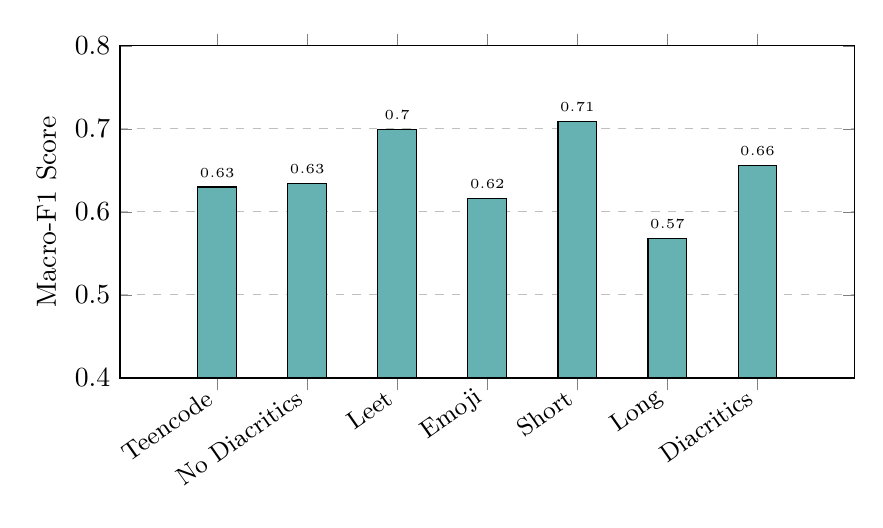
\begin{tikzpicture}
\begin{axis}[
    ybar,
    enlarge x limits=0.18,
    ylabel={Macro-F1 Score},
    symbolic x coords={Teencode,No Diacritics,Leet,Emoji,Short,Long,Diacritics},
    xtick=data,
    x tick label style={rotate=35,anchor=east,font=\small},
    nodes near coords,
    nodes near coords align={vertical},
    every node near coord/.append style={font=\tiny\bfseries},
    ymin=0.4, ymax=0.8,
    width=0.9\textwidth,
    height=5.8cm,
    bar width=14pt,
    ymajorgrids=true,
    grid style=dashed,
]
\addplot[fill=teal!60] coordinates {(Teencode,0.630) (No Diacritics,0.634) (Leet,0.699) (Emoji,0.616) (Short,0.709) (Long,0.568) (Diacritics,0.656)};
\end{axis}
\end{tikzpicture}
\caption{Macro-F1 performance comparison across noise and surface form categories.}
\label{fig:f1_by_surface}
\end{figure}

\subsection{Analysis of the 504 Blind-Spot Samples}
Table~\ref{tab:blind_spot_full} analyzes ground-truth label distributions for the 504 test comments missed simultaneously by all six neural backbones.

\begin{table}[H]
\centering
\caption{Class distribution of the 504 blind-spot test comments missed by all six neural backbones on ViHSD.}
\label{tab:blind_spot_full}
\begin{tabular}{lcc}
\toprule
Ground-Truth Class & Sample Count ($N$) & Percentage (\%) \\
\midrule
HATE & 185 & 36.7\% \\
OFFENSIVE & 180 & 35.7\% \\
CLEAN & 139 & 27.6\% \\
\midrule
\textbf{Total Blind-Spot} & \textbf{504} & \textbf{100.0\%} \\
\bottomrule
\end{tabular}
\end{table}

\begin{figure}[H]
\centering
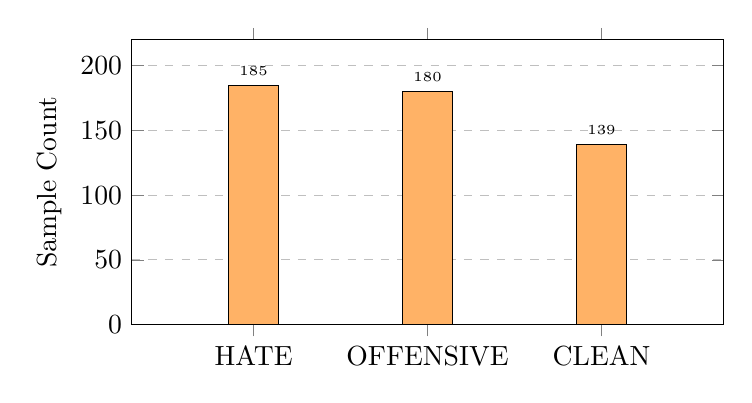
\begin{tikzpicture}
\begin{axis}[
    ybar,
    enlarge x limits=0.35,
    ylabel={Sample Count},
    symbolic x coords={HATE,OFFENSIVE,CLEAN},
    xtick=data,
    nodes near coords,
    nodes near coords align={vertical},
    every node near coord/.append style={font=\tiny\bfseries},
    ymin=0, ymax=220,
    width=0.75\textwidth,
    height=5.2cm,
    bar width=18pt,
    ymajorgrids=true,
    grid style=dashed,
]
\addplot[fill=orange!60] coordinates {(HATE,185) (OFFENSIVE,180) (CLEAN,139)};
\end{axis}
\end{tikzpicture}
\caption{Class distribution within the 504 blind-spot comments missed by all six neural backbones.}
\label{fig:blind_spot_dist}
\end{figure}

\subsection{Decision Change Analysis}
Table~\ref{tab:change_analysis_full} summarizes decision modifications introduced by Hybrid Fusion relative to AI-only argmax.

\begin{table}[H]
\centering
\caption{Summary of decision changes introduced by Hybrid Fusion relative to AI-only argmax ($n=9{,}158$).}
\label{tab:change_analysis_full}
\begin{tabular}{lcc}
\toprule
Metric / Category & Value ($N$) & Rate (\%) \\
\midrule
Total Changed Decisions & 91 & 0.99\% \\
Corrections (Wrong $\to$ Correct) & 44 & 48.4\% \\
Regressions (Correct $\to$ Wrong) & 31 & 34.1\% \\
Net Gain & +13 & +0.14\% \\
\midrule
ViHSD Changed Decisions ($n=6{,}680$) & 64 & 0.96\% \\
\bottomrule
\end{tabular}
\end{table}

\section{Experimental and Hardware Environment}
Table~\ref{tab:experimental_setup} outlines exact computational infrastructure, software versions, and training protocols.

\begin{table}[H]
\centering
\caption{Summary of experimental hardware, software dependencies, and training protocol configuration.}
\label{tab:experimental_setup}
\scriptsize
\setlength{\tabcolsep}{2pt}
\resizebox{\textwidth}{!}{%
\begin{tabular}{ll}
\toprule
Category & Configuration Details \\
\midrule
Hardware & NVIDIA GeForce RTX 4060 Laptop GPU (8 GB VRAM), Intel Core i7-13700H, 32 GB RAM \\
Operating System & Windows 11 Home 64-bit \\
Software Stack & Python 3.11.9, PyTorch 2.5.1, Hugging Face Transformers 4.46.3, scikit-learn 1.5.2 \\
Backbone Architecture & \texttt{microsoft/mdeberta-v3-base} (12-layer, 768-hidden, 12-heads, 278M parameters) \\
Precision \& Batch & Single-precision FP32, Evaluation Batch Size = 32 \\
Random Seed & Fixed seed 42 across all backbone training and bootstrap runs \\
Evaluated Datasets & ViHSD test split ($n=6{,}680$), Davidson test split ($n=2{,}478$), Mixed stream ($n=9{,}158$) \\
\bottomrule
\end{tabular}%
}
\end{table}

\subsection{Lexicon Leakage Audit}\label{subsec:lexicon_leakage}
Table~\ref{tab:lexicon_leakage} reports the overlap between lexicon entries and held-out train/validation/test splits. All lexicon entries originate from the training split only; no entry is sourced from validation or test.

\begin{table}[H]
\centering
\caption{Lexicon leakage audit across train/validation/test splits.}\label{tab:lexicon_leakage}
\scriptsize
\setlength{\tabcolsep}{2pt}
\resizebox{\textwidth}{!}{%
\begin{tabular}{lllll}
\toprule
Lexicon & Terms & Bad split rows & Test comment matches & Fired in test not train \\
\midrule
VI (\texttt{verified\_lexicon.csv}) & 668 & 0 & 13 & 0 \\
EN (\texttt{verified\_lexicon\_en\_combined.csv}) & 818 & 0 & 0 & 0 \\
\bottomrule
\end{tabular}%
}

\end{table}

\section{Complete List of Supplementary Tables}
\begin{enumerate}
\item Table~\ref{tab:langid_full} --- Language routing confusion matrix
\item Table~\ref{tab:langid_robustness} --- Language detection accuracy on clean held-out sets (ViNLI + Wortschatz)
\item Table~\ref{tab:langid_latency} --- Sequential latency breakdown for language routing
\item Table~\ref{tab:rule_ablation_full} --- Vietnamese Rule Engine component ablation study
\item Table~\ref{tab:rule_confusion} --- Standalone Rule Engine confusion matrix breakdown
\item Table~\ref{tab:rule_per_class} --- Per-class metrics for standalone Rule Engine
\item Table~\ref{tab:vi_backbones_full} --- Performance metrics for Vietnamese backbones (M1--M6)
\item Table~\ref{tab:en_backbones_full} --- Performance metrics for English backbones
\item Table~\ref{tab:roc_ap_full} --- Multi-class ROC-AUC metrics across backbones
\item Table~\ref{tab:fusion_full} --- Comprehensive decision fusion variants comparison
\item Table~\ref{tab:calibration_full} --- Calibration diagnostics (ECE, Brier score, NLL)
\item Table~\ref{tab:e2e_detailed_full} --- Full end-to-end pipeline benchmark results
\item Table~\ref{tab:e2e_per_lang} --- Language-stratified Hybrid E2E performance
\item Table~\ref{tab:e2e_per_label_full} --- Full stream class-wise performance metrics
\item Table~\ref{tab:e2e_confusion_full} --- Normalized confusion matrix for Hybrid E2E
\item Table~\ref{tab:significance_full} --- Paired statistical significance tests (Bootstrap \& McNemar)
\item Table~\ref{tab:error_overlap} --- Error overlap distribution across backbones
\item Table~\ref{tab:prior_reweighting} --- Class prior-reweighting oracle diagnostic
\item Table~\ref{tab:surface_full} --- Performance stratification across surface forms
\item Table~\ref{tab:blind_spot_full} --- Ground-truth class breakdown of 504 blind-spot samples
\item Table~\ref{tab:change_analysis_full} --- Summary of decision changes introduced by Hybrid Fusion
\item Table~\ref{tab:experimental_setup} --- Hardware, software, and protocol parameters
\item Table~\ref{tab:lexicon_leakage} --- Lexicon leakage audit across train/validation/test splits
\end{enumerate}

\end{document}
